\documentclass{beamer}

\usepackage[utf8]{inputenc}
\usepackage[useregional]{datetime2}
\usetheme{Madrid}


\title[Topological Insulators] %optional
{Topological insulator classification}

\subtitle{A short account}

\author[] % (optional, for multiple authors)
{
% \and M.~Jake\inst{1} 
M.~Lingfa\inst{1} \inst{2}}

\institute[CU] % (optional)
{
	\inst{1}%
	the Cavendish Laboratory
	%University of Cambridge
	\and
	\inst{2}%
	Gonville and Caius College\\
	University of Cambridge
}

\date[Part II 2020] % (optional)
{Research Review, \today}

\logo{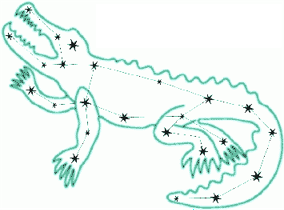
\includegraphics[height=1cm]{caplogo_l.png}}

% preamble

\AtBeginSection[]
{
	\begin{frame}
	\frametitle{Table of Contents}
	\tableofcontents[currentsection]
\end{frame}
}



\begin{document}
	% title page
	\frame{\titlepage}
	\begin{frame}
	\frametitle{Title page}
	Import the picture of a dirac cone.
	\end{frame}

	% table of contents
	\begin{frame}
	\frametitle{Table of Contents}
	\tableofcontents
	\end{frame}
	
	% section 1
	\section{Introduction}
	
	\begin{frame}
	\frametitle{Introduction}
	\end{frame}
	
	
	% section 2
	\section{Current Research}
	
	\begin{frame}
	\frametitle{Diffraction Methods}
	
	\end{frame}

	\begin{frame}
	\frametitle{Measurement Methods}
	
	\end{frame}
	
	% section 3
	\section{}
	
	
	\section{Diffraction grating}
	\begin{frame} 
	\frametitle{Diffraction grating}
	\end{frame}
	    
	
	
	\section{Conclusion}
	
	\begin{frame}
	\frametitle{Conclusion}
	\end{frame}
	

\end{document}